\documentclass[11pt]{article} %, twocolumn if need to be
\usepackage{geometry}
\geometry{a4paper}
\usepackage[parfill]{parskip}    		% Activate to begin paragraphs with an empty line rather than an indent
\usepackage{graphicx}					
\usepackage{times} % Times font
\usepackage{url,hyperref}	
\usepackage{amssymb}
\usepackage{amsmath}
\usepackage{xeCJK}
%\setCJKmainfont{SimSun}

\title{Chengyu Dictionary Documentation} % Project Documentation Title
\author{Xuefeng Luo \and Jingwen Li}
\date{}	% no date
\begin{document}
\maketitle

\section{Introduction}
\indent The Internet has promoted globalisation and along with it, the urge (or necessity) to be multilingual. Following this trend, Chinese learners worldwide have also increased in number. As an inseparable part of the Chinese language, \textit{Chengyu}, or the so-called "four-character idioms", is on the other hand difficult to master. One reason behind this is that there are simply so many of them and it is hard for a learner to learn them in chunks. Most of the \textit{Chengyu} are learned as they are encountered, which surely satisfies most learners practically, but not the hungry ones. To help the intermediate/advanced Chinese learners, we present this Chengyu Dictionary as an entry-point to tame these culturally rich beasts.\\
\\
\indent This paper is presented in the following structure:\\
Section 2 talks about the existing tools and a paper on translating Chengyu into English. Section 3 lists the project dependencies. Section 4 is about data processing, including preprocessing the corpora, translation difficulties and other lexicographic decisions made. Section 5 deals with the search mechanism with technical details. Then, in section 6, we present the user interface. Section 7 recorded the division of labor and section 8 is our discussion of this tool and vision for future improvements.

\section{Related Works}
The following are existing tools that share similar functions with our web application:
\begin{itemize}
\item Chengyu Dictionary provided by \textit{Chinese-Tools.com}\\
\textit{Chengyu Dictionary} is an online dictionary that provide pinyin, explanations in English (only for some entries) and detailed explanations in Chinese for 30000 Chengyu. The information provided in Chinese includes meaning, context(origin), example, synonyms, antonyms and even grammatical information. A user may search by pinyin or Chinese character input, but not English. The results are displayed in a list of links which lead to the entries' own page, where the above information are presented.\\
\\
Available at: https://www.chinese-tools.com/chinese/chengyu/dictionary\\
\item lists of Chengyu that are introduced on websites, for example \textit{List of 148 well-known Chengyu}, available at: https://www.saporedicina.com/english/list-chengyu/\\
There are a lot of similar resources like this on the Internet. They are mainly summaries of frequently encountered Chengyu by Chinese learners, so they differ individually. Upon further inspection, they are not listed in the most-frequent-to-least-frequent manner, but overall these are very common Chengyu. Information provided for each Chengyu includes Chinese characters, pinyin and meaning in English.\\
\end{itemize}
There is also a paper on translation strategies: \textit{A Study of Idiom Translation Strategies between English and Chinese}\\
This paper discussed the different strategies that are commonly used when translating idiomatic phrases, Chengyu in particular, into English. The four main strategies are: literal translation, free translation, abridged translation and borrowing translation. It also outlined the principles to live by when translating idioms.


\section{Project Dependencies}
A list of project dependencies used in this project (managed by Maven):
\begin{itemize}
\item Google Web Toolkit and Mojo's Maven Plugin for GWT  (gwt-maven-plugin, version 2.8.1)
\item mysql-connector-java(version 8.0.13)
\item GwtBootstrap3 and GwtBootstrap3-extras (gwtbootstrap3 and gwtbootstrap3-extras, version 0.9.4) for button group, button dropdown and multiple select.
\end{itemize}

\section{How to install}
To install our application, please follow the listed instructions:

\begin{enumerate}
  \item First, you need an environment where GWT can be deployed. At this moment, we are using Eclipse plus a GWT plugin where we retrieved it from Eclipse marketplace.
  \item Then, MySQL is needed in order to import our data.
  \item MySQL Workbench is optional but it helped comparing to MySQL command line tools.
  \item To import our data, you need to run data\_structure.sql file where our data structures and relations were stored.
  \item Then, you should first import Chengyu data from chengyu\_data.json file and tags data from tags.csv file, since there are foreign key dependencies.
  \item Then, you can import chengyu tags relations from chengyu\_tag.csv file.
  \item Following that, you need to go to DictionaryServiceImpl.java \\(located in chengyu.dict\textbackslash src\textbackslash main\textbackslash java\textbackslash com\textbackslash colewe\textbackslash ws1819\textbackslash server)\\ where database connection information was hard-coded in. Variables DB\_URL, USER and PASS need to be modified in order to make our program connect to the database.
  \item Please run the application through Eclipse.
  \item Open the page \text{http://localhost:8888/chengyudict} via a browser. We have tested and passed with Safari, Google Chrome and Firefox.
  \item Enjoy it!
\end{enumerate}

\section{Method}
\subsection{Pre-processing Steps}
\indent Currently, there was no ready-made data resources we could find. Therefore we found a Chinese Chengyu dictionary online resource, calculate all Chengyus' frequencies against the OpenSubtitles corpus as Dr.Johannes Dellert recommended, translated and tagged about 150 entries.

\subsubsection{Chengyu Data}
Available at: https://github.com/by-syk/chinese-idiom-db\\
These are Chengyu collected from the web, with a total count of 12976 entries. Each entry contains a Chengyu, its Pinyin. Other information includes explanation, origin and example sentences all in Chinese. However, some Chengyu are without origin and/or example sentences.

\subsection{Frequency of Chengyu}
\indent In order to allow Chinese Chengyu learner to learn the most commonly used Chengyu, we count each Chengyu against their occurrence in the OpenSubtitles corpus, which contains subtitles of films. Although Chengyu usage is limited in this corpus, we managed to obtain a general idea of how they are used. To count the occurrence of each Chengyu, we created a separate Python program located in the data folder named chengyu\_frequency.py.

\subsection{Data Format}
\indent The original data we retrieved was in Comma-separated Value (CSV) formatting. Since we wrote a Python program to count frequency and Python support JSON, and since MySQL also support JSON regarding importing data, we used JSON as our data format (see data.json in the data folder). As for tags and chengyu-tag relations, we kept the format as CSV format (tags.csv and chengyu\_tag.csv in the data folder) and for data structures, we remain in SQL format.

\subsection{Linguistic Problems}

\indent Written language and spoken language differ, film language is more so. Film subtitles might subject to the limitation of space and time, people may use them in a somewhat unnatural way. Therefore our choice of the OpenSubtitles corpus might have affected the frequency of Chengyu observed, depending on the genres of the film and the language used in the film. One improvement to be made could be to incorporate different kinds of corpora. But then another problem may emerge as the literature used might be old and language might be archaic. In this case, since OpenSubtitles contains contemporary language used in film subtitles, this corpus could be a good choice, other corpora of the same time period may be used for improvement of calculating frequency.\\

\subsection{Lexicographic Decisions}

\indent How to organise the entries. What information to include. \\

\subsection{Search Mechanism}

\indent We split our search function into two parts. The initial search and a tag filter.

In our initial search, we first determine which mode the user choose and pass target and mode variables to our search logic class. In this class, we already made SQL statement templates and inserted variables into those statement and request database to search.

After database returning back, we retrieved the data and parsed the data into an arraylist of Entries. Then, we used the pre-made function to filter the results and sent them to the front.

Intuitively, we wanted our filter function takes place in the front-end to be written by JavaScript as the industrial standards usually do. However, we found GWT having problems with this method where user interface was designed in Java and written JavaScript was actually very hard to step in. Thus, we moved our tag filter function back to Java. 

\subsection{Database}
\indent We are using MySQL which is the world's most commonly used and free relational database and it is easy to use and maintain.

To design our data tables, we follow first, second and third normalization where we eliminated all repeating records, partial dependency and transfer dependency. Thus, we have Chengyu table and Tags table and one more associate table which stores the relationships of Chengyu and Tags where we have IDs for both Chengyu and Tags as primary keys and foreign keys.

Figure 1 shows the relationships of our tables.

\indent a ERD of our table

\section{User Interface}

\subsection{Three Search Modes}
\indent To search a Chengyu, you can directly search it by typing in its Chinese characters. If you have forgotten the Chengyu and remember only a part of it, you can search the Chengyu by typing in one of the characters contained in the Chengyu. However, you'll have to go through the results to find your desired Chengyu. In addition you may also search in pinyin.

As for English mode, sometimes you may want to search a Chengyu which has a specific meaning. In this case you can type in its English meaning. For example if you want to search for Chengyu containing the meaning of \textit{mistake} in it, you may select English mode, type in \textit{mistake} and search.

To summarise, we designed these three search modes where you can search by Chinese, pinyin or English. The switches are displayed as a button group just above the input box, shown in Figure 1.

\begin{figure}[htbp]
\begin{center}
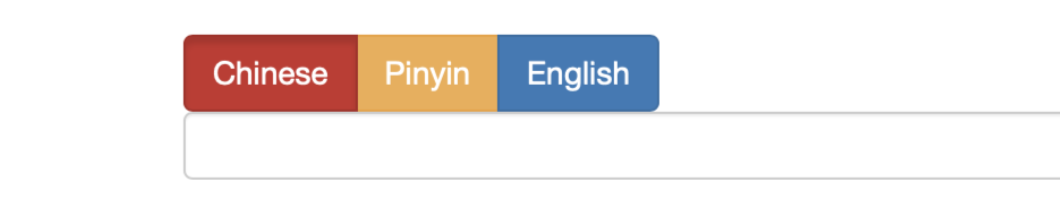
\includegraphics[width=10cm]{searchmode.png}%fig2
\caption{Three Search Modes}
\label{searchmode}
\end{center}
\end{figure}


\subsection{Tags}
\indent One interesting thing about Chengyu is that they love to use metaphors of animals, human body parts and numbers. Therefore we have character tags like \textit{numbers} and \textit{color} indicating these metaphors are incorporated in the Chengyu.

Another interesting thing is that there are certain patterns to form a Chengyu, such as "一心一意", "三天两头", "七上八下" where the first and third characters are all numbers. And "一生一世" is in the form of AXAY, where the first and third character are the same, and is also a number. Therefore this Chengyu has two tags: AXAY and numbers. Tags like \textit{AXAY}, \textit{AABB} are form tags.

Attitude is also important to Chengyu, a same meaning can be separated to different Chengyu regarding its attitude. For example, "臭味相投" and "志同道合" both mean similar people go together, but the former is used for bad persons such as gangsters and the later is used for normal people such as business partners. To further illustrate this point, let's continue with our \textit{mistake} example, if you performed the search mentioned above, you'll get three Chengyu: "将功赎罪", "万无一失" and "铸成大错". You may expect all of them to mean something negative as they are related to mistakes. In fact, the first two are quite the opposite. The first one makes up a mistake and the second indicates no mistakes are made, therefore they each have a positive tag. Tags like \textit{positive}, \textit{negative} are the sense tags.

That is why, we designed this tag filter to help people narrow-down all kinds of Chengyu. To perform a tag search, you may use any of the three mode and input some character/pinyin/English word (this is necessary for the search) and select the tags you want. Multiple selection is enabled. However, notice that we have only annotated around 150 Chengyu so there won't be many results if you select more than 2 tags at the same time. If you want to cancel you selection of a specific tag, just click it again and it will be unselected. You can either perform a tag search right from the beginning or narrow-down you search result by selecting tags later. Just press the search button again after your selection. The advanced search button works only as a label. \\
\\
Figure 2 shows a table of Chengyu tag examples and Figure 3 and 4 shows how it looks like in our application. 

\indent a table of chengyu tags example 唇齿相依,虎头蛇尾,狗仗人势,一心一意,三天两头, 七上八下, 臭味相投, 志同道合

\indent a screen shot of filter
\begin{figure}[htbp]
\begin{center}
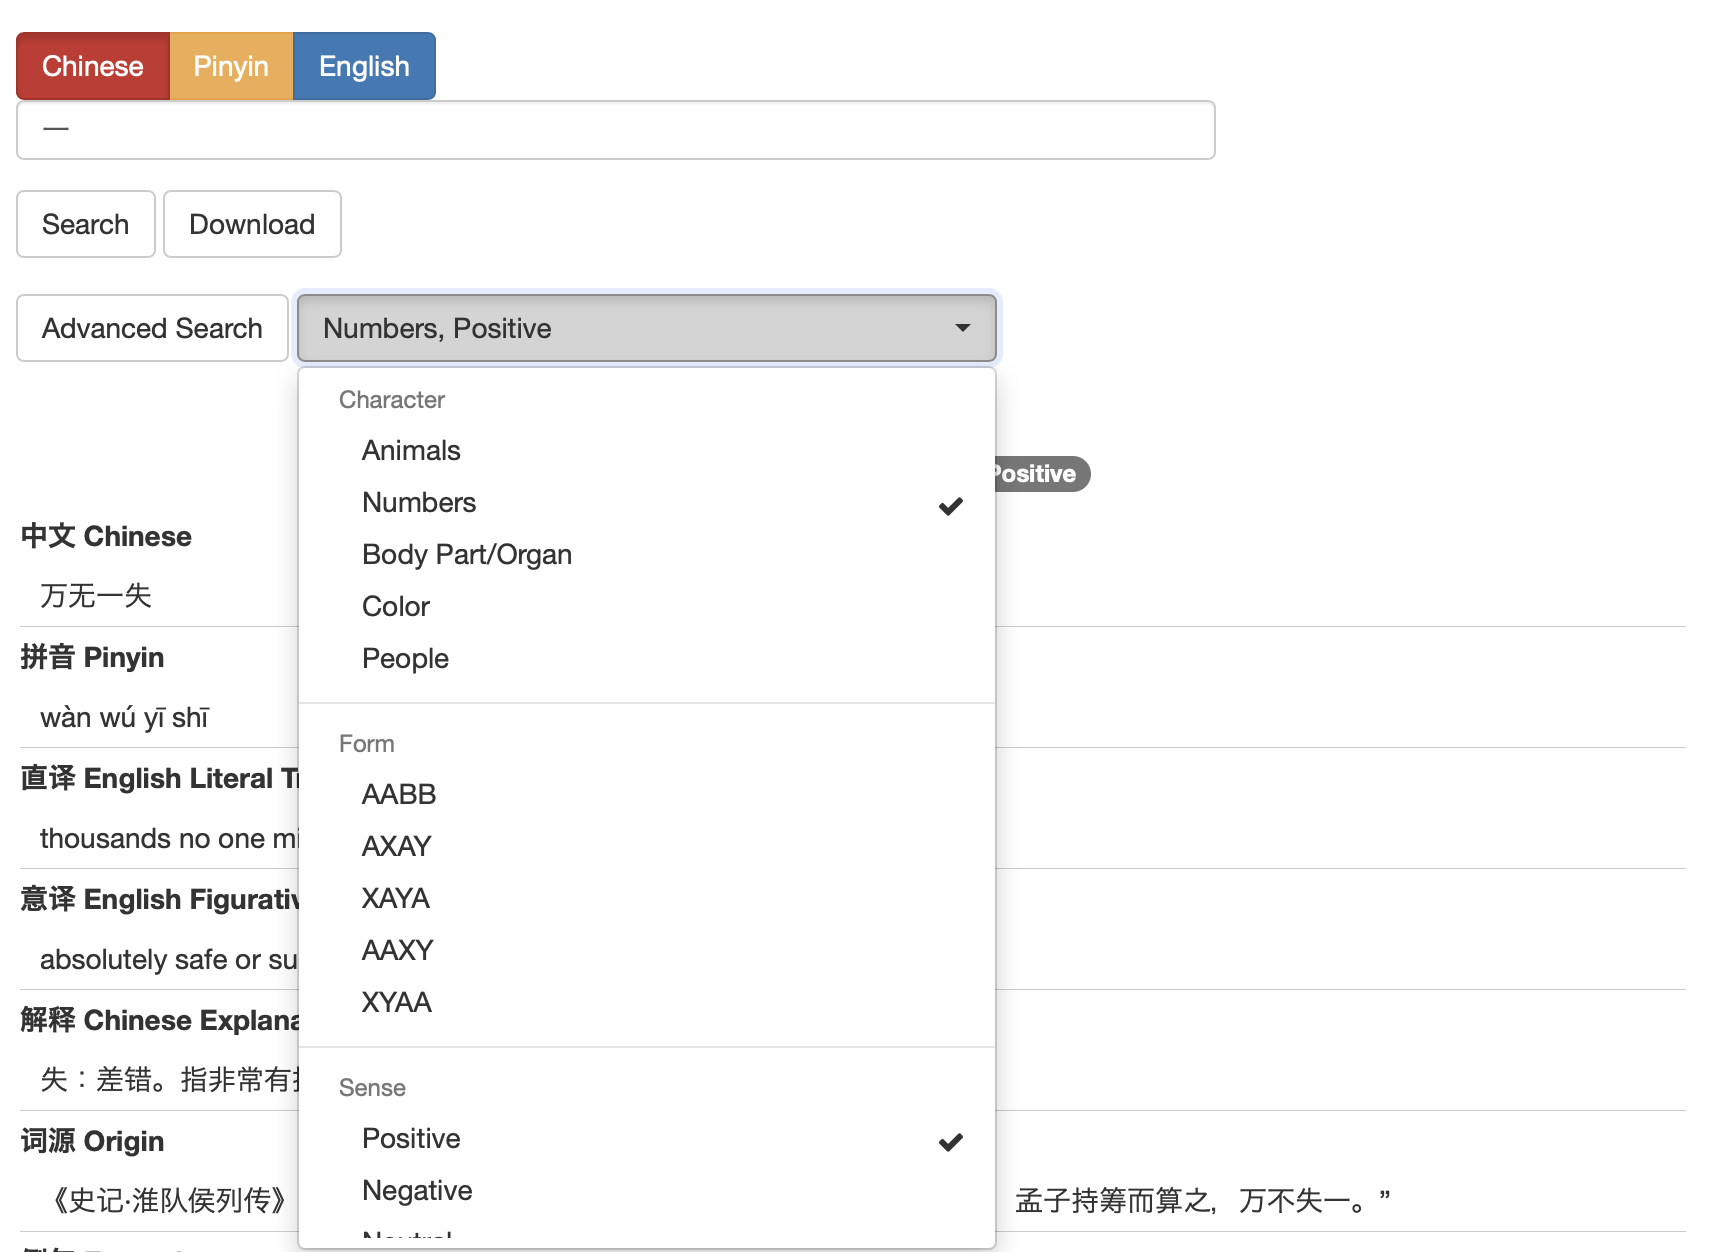
\includegraphics[width=14cm]{filter.png}
\caption{Tag Filter}
\label{default}
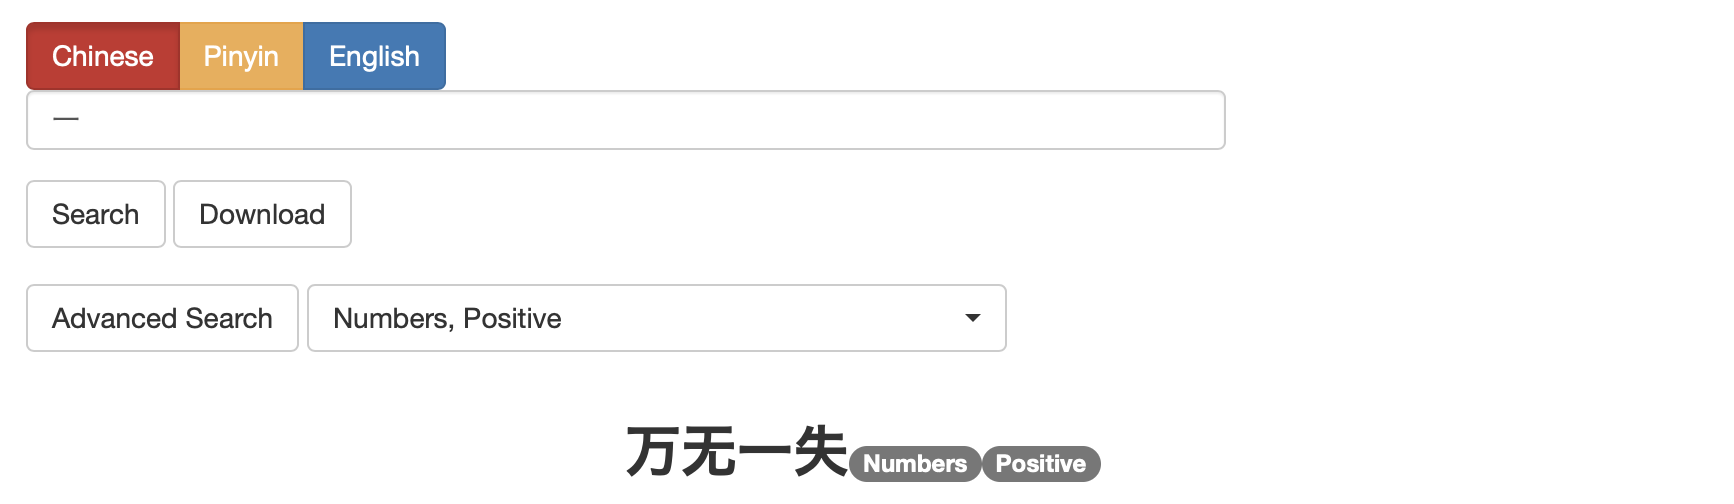
\includegraphics[width=14cm]{badge1.png}
\caption{Tags are displayed as badges attached to result title}
\label{default}
\end{center}
\end{figure}

\subsection{Results Display}

\indent Search results are displayed in the lower section of our page, shown as Figure 5, where each Chengyu takes a block and each column of information in the database takes a row in the block. Tags are attached as badges to the title.

\begin{figure}[htbp]
\begin{center}
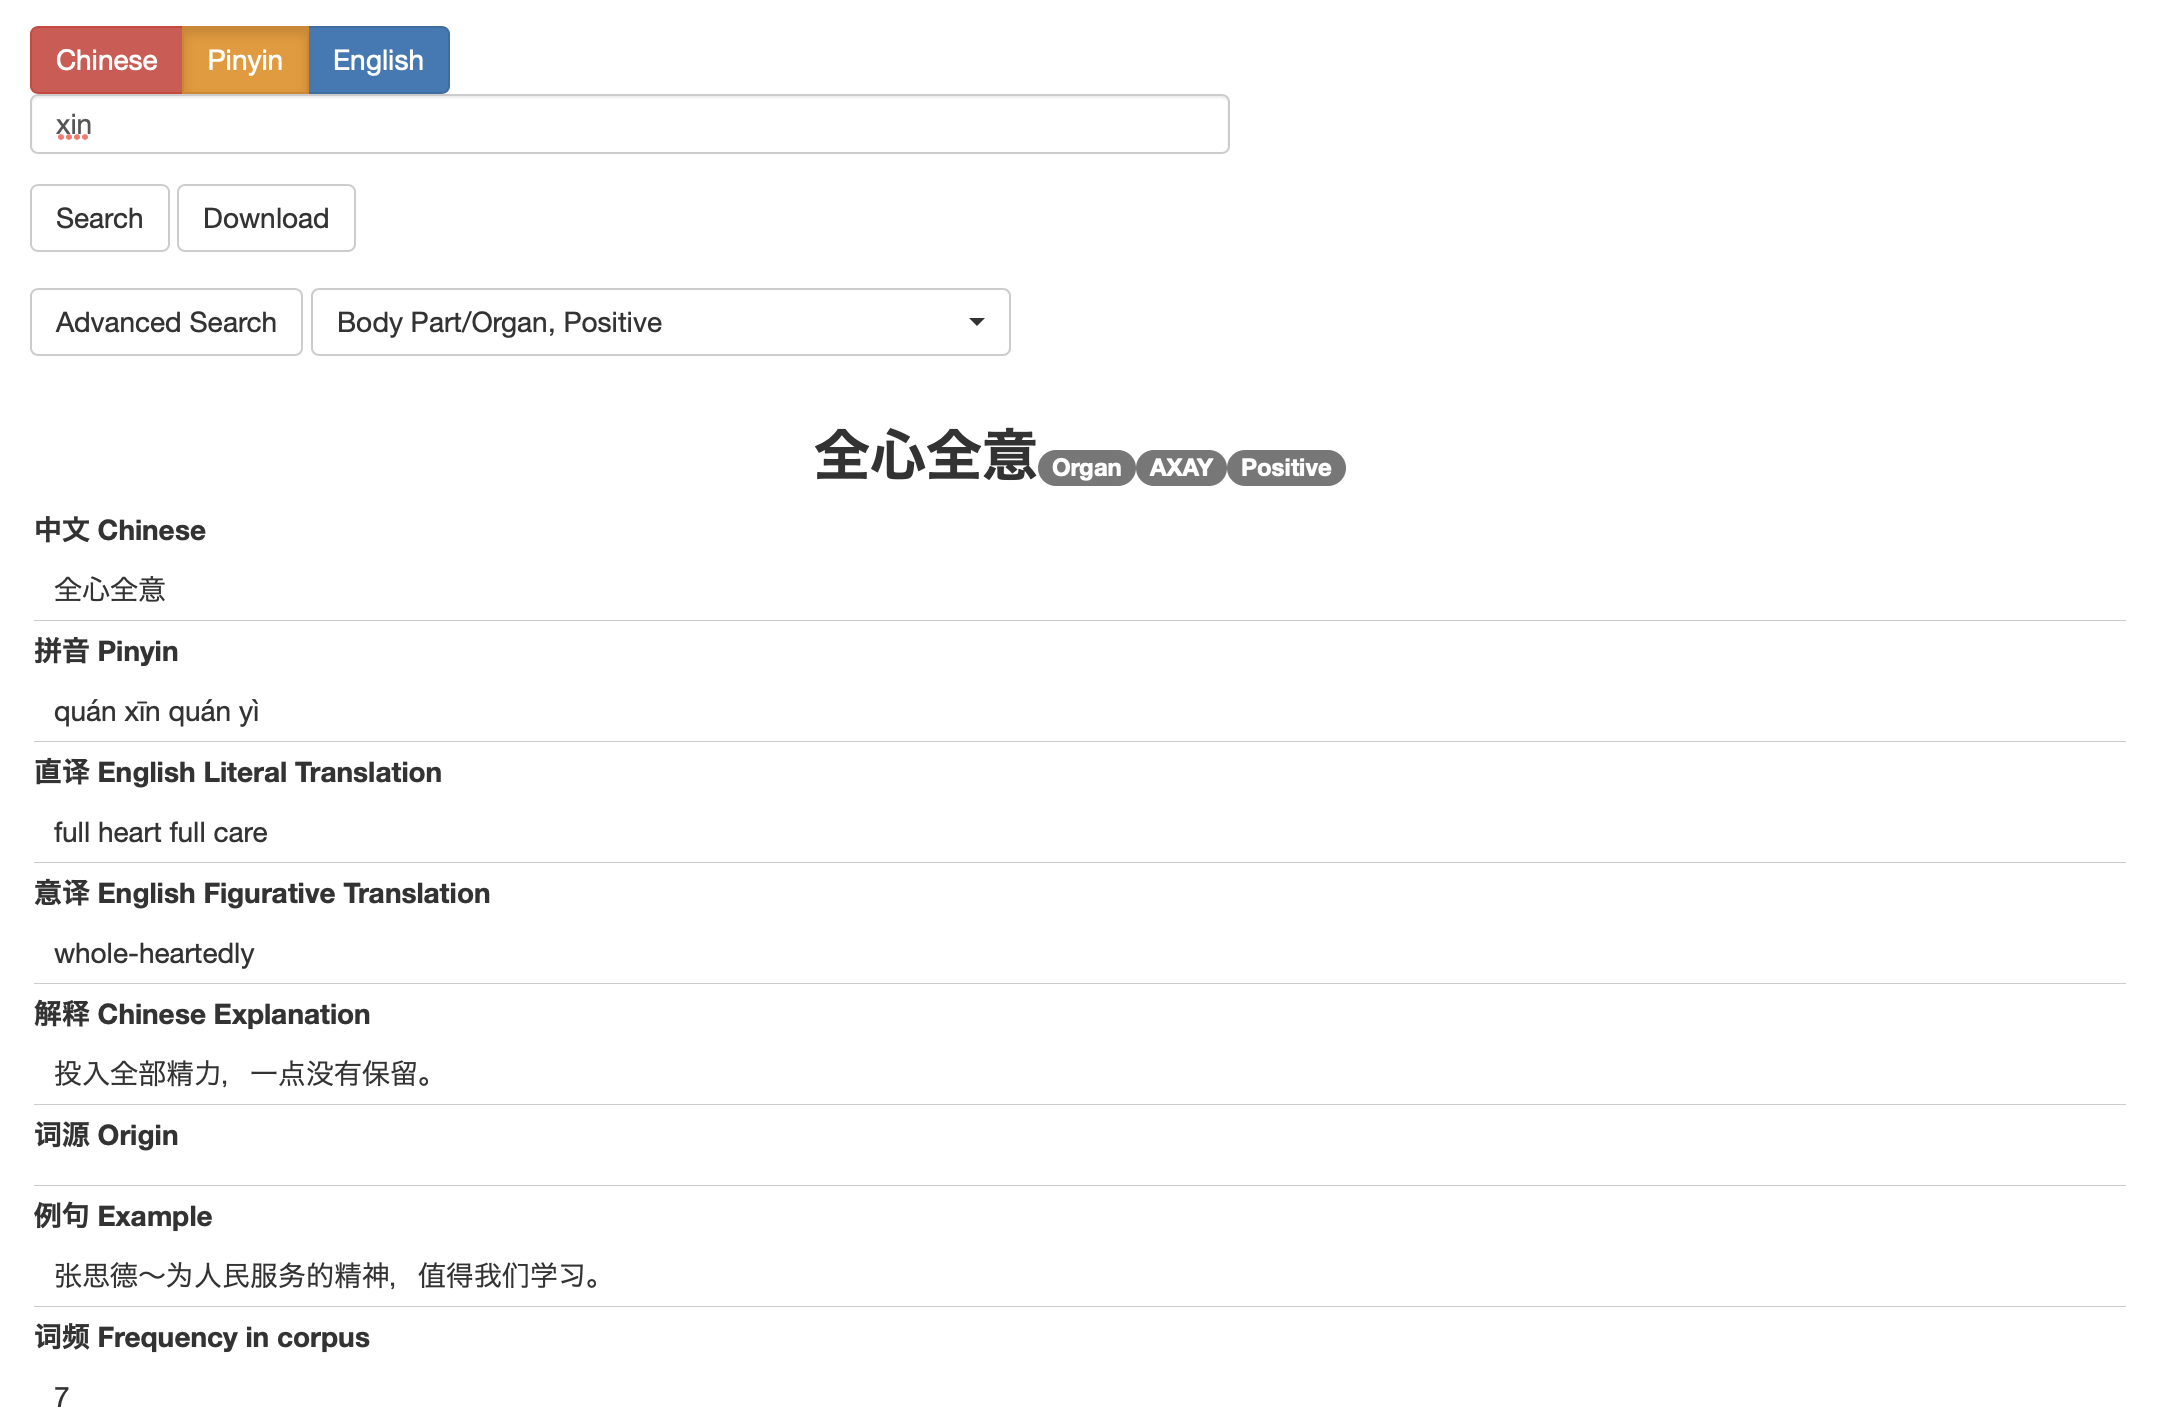
\includegraphics[width=15cm]{result.png}
\caption{Search result for pinyin search mode, input "xin", select tags "Body Part/Organ" and "Positive"}
\label{default}
\end{center}
\end{figure}

\subsection{Download}
You may want to download your current search results for future reference. This is performed by the download button. 

\section{Division of Labor}

\indent We worked as a team for the majority of the project parts. However, we do have specialties regarding what we are good at and what we are not. Therefore, we make a list of all sections with percentages of what we have done.

\begin{itemize}
    \item Database designs (Xuefeng 70\% and Jingwen 30\%)
    \item Front-end/client side coding (Xuefeng 50\% and Jingwen 50\%)
    \item Back-end/server side coding (Xuefeng 70\% and Jingwen 30\%)
    \item Data collection (Xuefeng 30\% and Jingwen 70\%)
    \item Project Report (Xuefeng 30\% and Jingwen 70\%)
\end{itemize}

\section{Discussion and Future Work}
\indent What we have accomplished with regard to the initial plan we set out. What didn't. I guess one thing is that we did not do the origin translation. Pinyin search.

\indent What could be improved given more time invested on the project. 

\bibliographystyle{abbrv}
\bibliography{refs}

\end{document}  